\section{Introduzione}
  \begin{frame}{Math packages}

  In LaTeX esistono due pacchetti diversi, i quali forniscono svariate estensioni per il miglioramento della struttura informativa e della stampa di documenti che contengono formule matematiche:

    \begin{itemize}
      \item<1-> Pacchetto \texttt{\textcolor{blue}{amsmath}}
      \item<2-> Pacchetto \texttt{\textcolor{blue}{amssymb}}
	  \item<3-> \mintinline{latex}{\usepackage{amsmath, amssymb}}
    \end{itemize}

    \begin{itemize}
      \item<4-> Formule ``in linea'' $a^2 + b^2 = c^2$
      \item<5-> Formule ``in display''
      \begin{itemize}
        \item[]<5-> \begin{equation} e^{i\pi}+1=0 \end{equation}
      \end{itemize}
    \end{itemize}
    
    \begin{textblock*}{5cm}(9cm,4cm)
      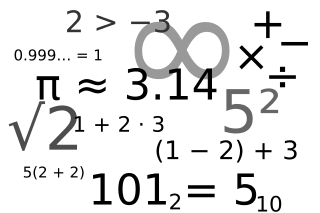
\includegraphics[scale=0.25]{math_symbols}
    \end{textblock*}

\end{frame}
